%Resume Hello word python dan identation

%Kelompok 2 D4 TI / 2B

%Alwan Suryansah				1164033 
%Dinda Ayu Pratiwi				1164034
%Kurnia Sandi					1164042
%Teduh Sanubari					1164054
%Wildan Khaustara Wijaksana		1164058

\documentclass[12pt]{article}
\usepackage{graphicx}    

\begin{document}
\section{Apa itu Pyton?}

\subsection{Journal JCONES}
	Tulisan ini mendiskusikan pengertian python , python adalah sebuah bahasa pemrograman model skripsi atau ( scripting language) terorientasi objek. atau bisa juga di artikan sebagai bahasa pemrograman yang freeware atau perangkat bebas , tidak ada batasan dalam penyalinan atau mendistribusikan . yang di dalamnya terdapat source code , debugger dan profiler \cite{perkasa2014rancang}.
	
\subsection{Dierbach, Charles}
Bahasa pemrograman Python telah dengan cepat mendapatkan popularitas selama beberapa tahun terakhir sebagai bahasa pilihan untuk kursus CS1. Beberapa perkiraan menyebutkan bahwa penggunaannya meningkat empat puluh persen per tahun. Sejauh 2006 ada laporan peningkatan yang signifikan dalam kepuasan siswa dan instruktur dengan mendesain ulang kursus pengantar untuk menggunakan kesederhanaan Python daripada kompleksitas bahasa seperti Java\cite{dierbach2014python}.

\subsection{Computing, Jurnal ULTIMA}
Python merupakan bahasa pemrograman open source yang banyak digunakan untuk menangani beberapa jenis masalah dalam pemrograman. Python banyak digunakan untuk meningkatkan kualitas perangkat lunak, produktivitas pengembang, portabilitas program, dan integrasi komponen. Python digunakan oleh setidaknya ratusan ribu pengembang di seluruh dunia dalam bidang-bidang seperti scripting internet, pemrograman sistem, user interface, kustomisasi produk, pemrograman numerik, dan banyak lagi\cite{computingaplikasi}.

\subsection{Herho, Sandy Hardian Susanto}
Python merupakan bahasa pemrograman tingkat tinggi yang dewasa ini telah menjadi standar dalam dunia komputasi ilmiah. Python merupakan bahasa pemrograman open source multi-platform yang dapat digunakan pada berbagai macam sistem operasi (Windows, Linux, dan MacOS). Selain itu, Python juga merupakan bahasa pemrograman yang fleksibel dan mudah untuk dipelajari. Program yang ditulis dalam Python umumnya lebih mudah dibaca dan jauh lebih ringkas dibandingkan penulisan program dalam bahasa C atau Fortran. Python juga memiliki modul standar yang menyediakan sejumlah besar fungsi dan algoritma, untuk menyelesaikan pekerjaan seperti mengurai data teks, memanipulasi dan menemukan file dalam disk, membaca / menuliskan file terkompresi, dan mengunduh data dari server web. Dengan menggunakan Python, para programmer juga dapat dengan mudah menerapkan teknik komputasi tingkat lanjut, seperti pemrograman berorientasi objek\cite{herho2018tutorial}.

\subsection{Rizky, Gusti Yudhistira and Anbarsanti, Nurfitri and others}
Bahasa python sendiri adalah Bahasa pemrograman yang bersifat freeware. Maksudnya adalah tidak memiliki batasan dalam melakukan penyalinan atau pemakaiannya yang lengkap dengan source codenya, debugger, dan profiler, interface service, fungsi system GUI, dan basis datanya sehingga dapat membuat python menjadi basaha asli raspberry. Python sendiri memiliki beberapa fitur. Seperti memiliki kepustakaan yang luas dengan modul-modul siap pakai untuk berbagai macam keperluan\cite{rizky2016desain}. 

\section{Membuat "Hello World" dengan Pyton}
"Hello World" adalah kalimat sakral yang pertama kali dimunculkan menggunakan bahasa pemrograman tertentu dalam sistem. Para coder dari tahap beginner hingga tingkat expert pun pasti hal yang pertama ia lakukan adalah memunculkan "Hello World" di sistem. Karena prinsip utama dalam pemrograman adalah bagaimana memunculkan apa yang kita tulis atau kita buat dengan bahasa pemrograman tertentu ke sebuah layar atau sistem baik dengan atau tanpa data.
Berikut ini adalah code untuk menampilkan "Hello World" di layar menggunakan bahasa pemrograman Python

\begin{verbatim}
>>> print('hello world')
hello world
\end{verbatim}

\subsection{Membuat "Hello World" dengan menggunakan Token pada bahasa Python}
Pada bahasa python terdapat kalimat "Hellow World" di layout awal untuk melihat apakah ada terdapat error pada halaman itu.apa bila tidak terdapat error "Hello World" akan muncul di halaman awan atau layout awal . dengan menggunakan Token instance mewakili unit teks seperti kata,kalimat, atau dokumen, dan didefinisikan oleh (sebagian)pemetaan dari nama properti kenilai.Sebagai contoh,properti Text digunakan untuk menyandikan token\cite{bird2004nltk}:

\begin{verbatim}
>>> dari nltk.token impor *
>>> Token (TEXT = "Hello World!")
<Hello World!>
\end{verbatim}

Secara umum, tugas pemrosesan bahasa diformulasikan sebagai anotasi dan transformasi yang melibatkan Token. Secara khusus, setiap tugas pemrosesan membutuhkan token dan meluasnya untuk memasukkan informasi baru. Modifikasi ini biasanya monotonik; baru informasi ditambahkan tetapi informasi yang ada tidak dihapus atau diubah. Jadi, token berfungsi sebagai papan tulis, dimana informasi tentang sepotong teks disusun. Arsitektur ini berbeda dengan yang lainnya arsitektur pipa khas di mana setiap pemrosesan keluaran tugas membuang informasi masukannya. Kita memilih pendekatan papan tulis di atas pipa pendekatan karena memungkinkan lebih banyak fleksibilitas kapan menggabungkan tugas ke dalam satu system\cite{bird2004nltk}.

\subsection{Membuat "Hello World" dengan Pyton menurut Perkel, Jeffrey M}
Bahasa pemrograman Python lebih mudah dinyatakan, pengguna tidak harus menentukan variabel mana yang akan menyimpan angka atau teks, misalnya. Latihan pemrograman klasik Percetakan 'Hello, world!' ke layar sesederhana mungkin dengan Python - ketikkan saja

\begin{verbatim}
print ("Hello, world!”)
\end{verbatim}
pada prompt Python dan tekan Enter\cite{perkel2015programming}.

\subsection{Membuat "Hello World" Menurut Buku Logika algoritma dan implementasinya dlm bahasa python di gnu/linux}
Python merupakan salah satu bahasa pemrograman tingkat tinggi dengan tipe bahasa interpreted karena program-program Python langsung dieksekusi oleh interpreter tanpa harus melalui tahap kompilasi. Python dapat dijalankan dengan dua cara, yakni:
\begin{enumerate}
\item Mode command-line
Dengan mode ini, program dapat dilakukan dengan memanggil interpreter, kemudian memberi statement Python dan interpreter akan menampilkan hasil, sebagai contoh:
\begin{verbatim}
bash-2.05a$ python
Python 2.1.3 (#1, Apr 20 2002, 10:14:34)
[GCC 2.95.4 20011002 (Debian prerelease)] 
on linux2 Type "copyright", "credits" or 
"licence" for more information.

>>> print 1+1
2
>>> print "Hello World!"
Hello World!
\end{verbatim}

\item Mode Script
Mode ini dilakukan dengan cara menuliskan keseluruhan program dalam file, kemudian interpreter akan mengeksekusi seluruh isi dari file. File seperti ini dinamakan script. Sebagai contoh, sebuah file yang ditulis dengan text editor dan diberi nama script01.py memiliki isi sebagai berikut:
\begin{verbatim}
print 1+1
\end{verbatim}
Dengan perjanjian bahwa file yang berisi program Python diberi nama dengan ekstensi .py. Eksekusi dari program dengan mode ini dapat dilakukan dengan cara sebagai berikut:
\begin{verbatim}
$ python script01.py
2
Contoh 1:
# -------------------
# Program Sederhana
# by Ema dan Wawan
# -------------------
print "I Like Python"

Contoh 1.1:
# -------------------
# Program Sederhana
# by Kurnia Sandi
# -------------------

print "Hello World!"
\end{verbatim}
Catatan: Python tidak membutuhkan titik koma (semicolon) di belakang statement. Semicolon di sini sifatnya optional sehingga bisa digunakan, tetapi juga boleh tidak dipakai\cite{utami2004logika}.
\end{enumerate}

\subsection{Membuat "Hello World" Menurut Gario, Marco and Micheli, Andrea}
Python merupakan salah satu bahasa pemrograman tingkat tinggi akan tetapi python memiliki code atau syntax yang singkat , dan menggunakan bahasa C, C++, maupun Java, yakni:


\begin{verbatim}
from pysmt.shortcuts import * 
from pysmt.typing import INT 
 hello = [Symbol(s, INT) for s in "hello"] 
 world = [Symbol(s, INT) for s in "world"] 
 letters = set(hello+world) 
 domains = And([And(GE(l, Int(1)), 
 LT(l, Int(10))) for l in letters]) 
 sum_hello = Plus(hello) # n-ary operators can take lists 
 sum_world = Plus(world) # as arguments 
 problem = And(Equals(sum_hello , sum_world),
 					Equals(sum_hello , Int(25))) 
 formula = And(domains , problem) 
 print("hello world:") 
 print(World) 
 
 model = get_model(world , solver_name="z3") # Try msat 
 
 if model: print(model) 
 else: print("No solution found")

\end{verbatim}

\subsection{Menyapa Program Hello World Menurut Sweigart, Al}
Itu tradisional bagi pemrogram untuk membuat tampilan pertama mereka Hello World! di layar. Anda akan membuat program Hello World Anda sendiri sekarang\cite{sweigart2016invent}.
\begin{verbatim}
1. # Program ini menyapa dan menanyakan nama saya.
2. print('Hello world!')
3. print('Siapa nama Anda?')
4. myName = input ()
5. print('Ini baik untuk bertemu dengan Anda,' + myName)
\end{verbatim}

\subsection{Sochat, Vanessa}
Misalnya, untuk mengetahui lokasi eksak yang tepat yang ditulis dalam program yang berbeda bahasa ming untuk menghasilkan output "Hello World," kita bisa lakukan pembanding lebih lanjut dengan isinya, atau lakukan panggilan bahasa agnostik dengan melakukan atrace of system calls. Maka dari itu jenis penilaian yang memungkinkan untuk organisasi aplikasi dan aksesibilitas adalah hal yang terpenting\cite{sochat2018scientific}.

\subsection{Parra, Alfredo}
Seperti gambar pada di bawah ini untuk memunculkan "Hello World" pada scrip python.

\begin{figure}
\begin{center}
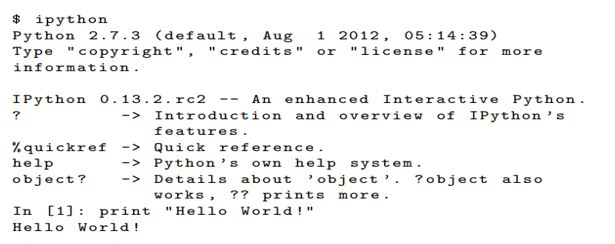
\includegraphics[width = 10cm, height= 7cm]{coding.jpg}
\caption{gambar1} 
\end{center}
\end{figure}


Keterangan:
\begin{enumerate}
\item Kerangka interaktif yang disempurnakan.
\item menggunakan python versi 2.7.3.
\item (?) adalah introduction dan overview di python features.
\item quickref untuk quick references .
\item help berfungsi untuk system help dalam python .
\item in [1]: print "hello world!" adalah yang akan muncul di layout sesuai yang di tuliskan.
\item hello world adalah loyout yang muncul setelah di ketikkan di kodingan menggunakan bahasa python.
\end{enumerate}

itulah keterangan dari pada gambar1 \cite{parra2017scripting}

 
\section{Pengertian Identation pada Pyton}

\subsection{Barry, Paul}
Python menggunakan prinsip yang berbeda. Program Python terstruktur melalui indentasi, yaitu blok kode ditentukan oleh indentasinya. Oke, itulah yang kami harapkan dari kode program apa pun, bukan? Ya, tetapi dalam kasus Python itu adalah persyaratan bahasa bukan masalah gaya. Prinsip ini membuatnya lebih mudah untuk membaca dan memahami kode Python orang lain \cite{barry2016head}.

\subsection{Kurniawan, Halim and Setiyono, Budi and Isnanto, R Rizal}
Bahasa pemograman Python adalah bahasa pemograman yang mudah dibaca dan terstruktur, hal ini karena di gunakannya sistem identasi. Yaitu memisahkan blok - blok program susunan identasi. Jadi untuk memasukan sub - sub program dalam suatu blok, sub - sub program tersebut diletakkan satu atau lebih spasi dari kolom suatu blok program itu \cite{kurniawan2011aplikasi}.

\subsection{Burt, Simon}
penyorotan sintaks dalam fitur indentasi khusus untuk Python, Tidak seperti kebanyakan Halnya yang Ada di dalam bahasa pemrograman, Python tidak biasa dalam hal itu menggunakan indentasi, berdasarkan sintaks yang di gunakan untuk membatasi blok kode. Pemrogram ini akrab dengan bahasa lain yang menggunakan delimiter, seperti kurung kurawal {and} untuk mengidentifikasi blok baru dan mungkin akan menemukan kebingungan ini pada awalnya, tetapi dengan cepat menjadi normal\cite{burtusing}.

\subsection{MUTHOA, MUHAMMAD FARIS}
Bahasa pemograman Python yaitu bahasa pemograman yang mudah dibaca dan terstruktur, karena dalam Python digunakannya sistem indentasi/spasi yaitu memisahkan blok-blok program dengan susunan indentasi/spasi. Python sendiri memiliki sedikit perbedaan cara penulisan kode program dengan bahasa pemrograman lainnya, yakni di Python kita hanya menggunakan spasi sebagai pemisah blok program yang biasa disebut sebagai Indentasi. Kalau pada bahasa pemrograman yang lain seperti C/Java menggunakan tanda kurung sebagai pemisah blok program\cite{muthoa2017sistem}.

\subsection{Miftakhuddin, Mukhammad and Suadi, Wahyu and Pratomo, Baskoro Adi}
Identation Yaitu adalah memisahkan blok `blok program susunan identasi. Jadi untuk memasukan sub -sub program ke dalam suatu blok, sub sub program tersebut diletakkan satu atau lebih spasi dari kolom suatu blok program(tulisan yang menjorok kearah kanan. hal ini karena digunakannya sistem indentasi, identasi digunakan sebagai blok kode pada pernyataan seperti if, while, dan for\cite{miftakhuddinimplementasi}. 

\subsection{Kristjan, Arumae and Sarah, Myhre and Cassian, Olschewski}
Indentasi seperti lekukan ekspresi yang bersarang, merupakan hal penting dalam memproduksi skrip Python yang terbaca. Persyaratan indentasi yang ditegakkan Python secara khusus mengurangi ruang untuk kesalahan saat pengembang bekerja dengan basis kode tertentu. Selanjutnya, persyaratan dalam membuat kode yang dihasilkan umumnya lebih mudah dibaca dan dengan demikian lebih mudah dipelihara\cite{kristjansoccer}.


\section{Error yang Muncul serta Solusinya}


\section{Kesimpulan}

\end{document}


